% \documentclass[linenumbers,twocolumn]{aastex631}
\documentclass[linenumbers]{aastex631}

% Packages
\usepackage[utf8]{inputenc}
\usepackage{graphicx}
\usepackage{amsmath}
\usepackage{amssymb}
\usepackage{enumitem}
\usepackage{ulem}
% \usepackage{hyperref}

% Editing commands
\newcommand{\mm}[1]{{\textcolor{purple}{\bf #1}}}

% Make upright subscripts and superscripts in Mathmode.
\def\subinrm#1{\sb{\mathrm{#1}}}
{\catcode`\_=13 \global\let_=\subinrm}
\mathcode`_="8000
\def\supinrm#1{\sp{\mathrm{#1}}}
{\catcode`\^=13 \global\let^=\supinrm}
\mathcode`^="8000
\def\upsubscripts{\catcode`\_=12 } \def\normalsubscripts{\catcode`\_=8 }
\def\upsupscripts{\catcode`\^=12 } \def\normalsupscripts{\catcode`\^=7 }

\newcommand{\vdag}{(v)^\dagger}
\newcommand\aastex{AAS\TeX}
\newcommand\latex{La\TeX}

% Title
\shorttitle{The Internal Shocks of GRB030329}
\shortauthors{Michael Moss}

\begin{document}

\upsubscripts
\upsupscripts

\title{Internal Shocks as the Mechanism for the Afterglow Behavior of GRB030329}

\author{Michael Moss}
\affiliation{The Department of Physics, The George Washington University, 725 21st NW, Washington, DC 20052, USA}
\affiliation{Astrophysics Science Division, NASA Goddard Space Flight Center, Greenbelt, MD 20771, USA}
\affiliation{Sorbonne Universit\'e, CNRS, UMR 7095, Institut d'Astrophysique de Paris, 98 bis Arago, 75014 Paris, France}


\correspondingauthor{Michael Moss}
\email{mikejmoss3@gmail.com}


\section{Abstract}

The acceleration mechanisms and emission processes which produce the observed prompt emission of Gamma-Ray Bursts (GRBs) are still under debate. The dominant emission component of the prompt emission is commonly described as synchrotron radiation from a population of electron accelerated by internal shocks or perhaps magnetic reconnection events. In other models, the emission can be shown to be purely thermal in nature. 

GRB030329 is a nearby (z$\sim 0.1685$) GRB with prompt and intense afterglow emission. The afterglow light curve shows a power law decay with time ($\alpha_1 = 0.9$) with a break at $\sim0.5$ days ($\alpha_1 = 1.9$). Interestingly, following this break the afterglow light curve displays two, possibly three or more, bumps (see Fig. \ref{fig: GRB030329 light curves}). Each bump increases the brightness of the light curve but does not change the power law index. These bumps occur on a timescale shorter than the observed time ($\Delta t / t \lesssim 1$). The first of these bumps occurs at $t_{bump}\sim 1$ day and has a rise time of $\Delta t_{bump}\sim0.3$ days. \citet{2003Natur.426..138G}, investigate the possible mechanism which may have caused these bumps, assuming the break at $\sim 0.5$ days is the jet break. The first possibility is that the circum-burst medium increases with radius in discrete steps. Such a density profile is quite unexpected. However, if such a density profile is produced, the bump features in the light curve could be produced, but are expected to be much smaller fluctuations in the X-ray light curve. A second possibility is the so-called ``patchy shell'' model, where the energy per unit solid angle injected in the GRB outflow is not constant. However, if we interpret the break in the light curve as the jet break, this means the whole emitting surface of the ejecta is visible. In this case, the non-uniformity of the energy per solid angle should be negligible. The final and most promising option considered is the ``refreshsed shocks'' model. We consider the assumption that the break at $\sim 0.5$ days is the jet break to be true and use a simplified model where the ejecta is emitted as shells of material to follow the evolution of the ejecta in the circum-burst medium. The aim is not to fit our results to data, but to investigate the viability of the internal shock model as a mechanism to explain the observed late time behavior.

We find that the bumps in the afterglow light curve of GRB030329 can be recreated if the central engine ejects slowly moving material ($\Gamma_{slow}~10$) sometime after the main prompt emission (see Fig. \ref{fig: simulated lorentz dist} and \ref{fig: simulated light curves}). We show that even if the slow material is ejected with a spread of Lorentz factors, internal shocks will naturally normalize the Lorentz factor of the slow material so that the spread will be small, $\Delta\Gamma_{slow}/\Gamma_{slow}\lesssim0.1$ (see Fig. \ref{fig: simulated lorentz dist}). A narrow distribution of Lorentz factors at the time of collision with the external shock is necessary to satisfy the observed $\Delta t / t \lesssim 1$ condition since $\Delta t / t \approx (8/3) \Delta \Gamma_{slow} / \Gamma$.

We do not claim that internal shocks must be the dominant acceleration mechanisms for the prompt emission. 

Due to the slow velocity of this later ejected material, the internal shocks of the slow material will occur at small radii, close to the central engine. This would indicate that the magnetization close to the central engines of GRBs is sufficiently low to allow for internal collisions or, alternatively, an evolution to lower values of the magnetization close the central engine.

\begin{figure}[!ht]
    \centering
    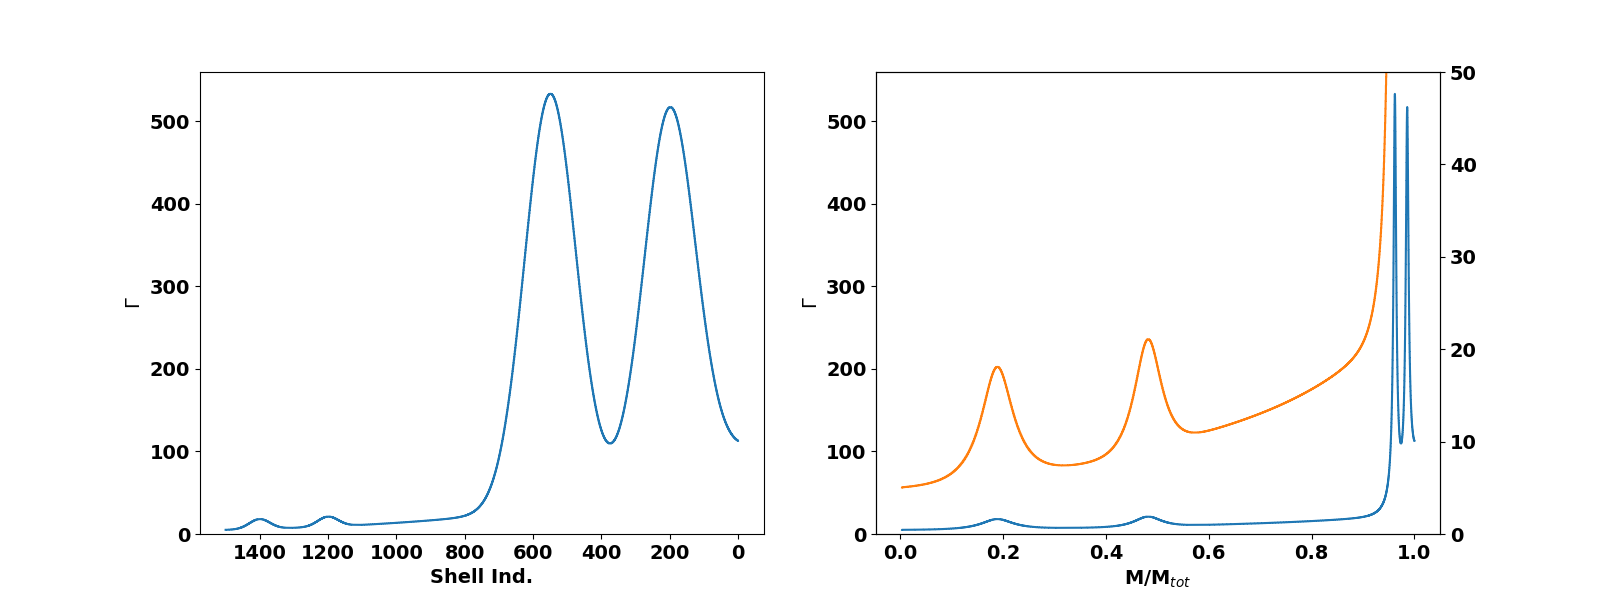
\includegraphics[width=1\textwidth]{figures/22-03-09-gauss-inject-with-zoom-T0.png}
    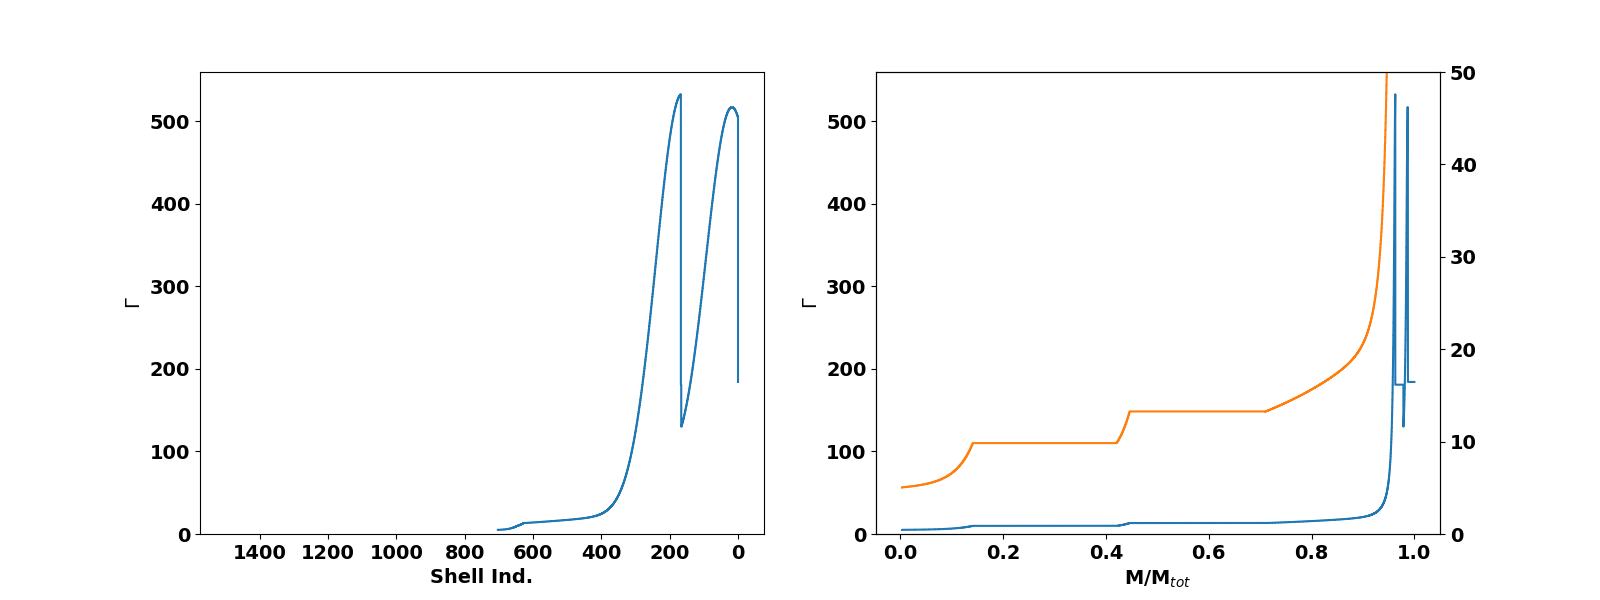
\includegraphics[width=1\textwidth]{figures/22-03-09-gauss-inject-with-zoom-TLater.png}
    \caption{The Lorentz distribution for the simulation at two times. The top two plots display the injected Lorentz distribution ($t = 0$ sec). The bottom two plots display the Lorentz distribution at a later time after many internal shocks have occurred. The orange curve is a zoom in of the blue curve to clearly show the behavior of the slower material. Left) the Lorentz factor of each shell in the simulation plotted against the shell number. Right) the Lorentz distribution of each shell plotted against the mass of each shell (displayed as the fraction of the total ejecta mass). The two large Gaussian curves are responsible for the double-peaked prompt emission while the much slower material ejected at later times collides with and re-energizes the external shocks, creating the late time bumps in the afterglow light curve (see Fig. \ref{fig: simulated light curves}).}
    \label{fig: simulated lorentz dist}
\end{figure}

\begin{figure}[!ht]
    \centering
    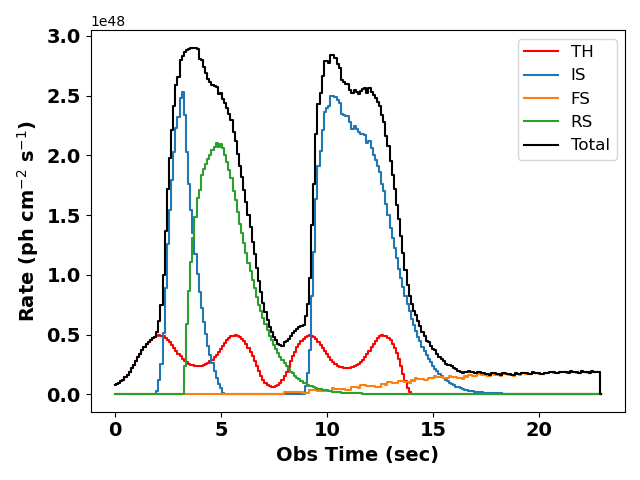
\includegraphics[width=0.49\textwidth]{figures/22-03-08-prompt.png}
    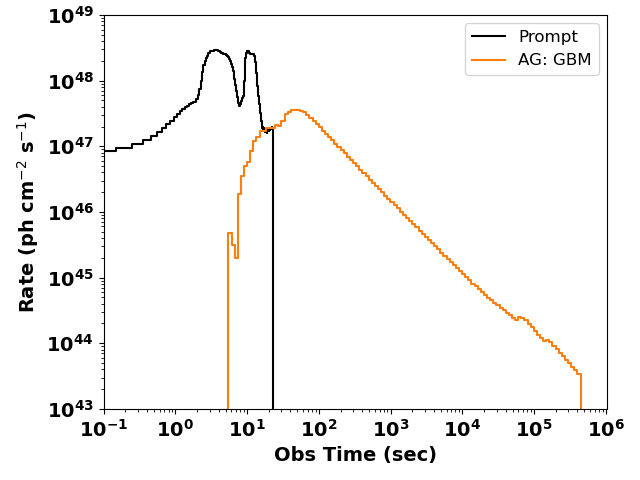
\includegraphics[width=0.49\textwidth]{figures/22-03-08-aftglow.png}
    \caption{Displayed are the light curves produced in the simulations assuming an injected Lorentz distribution of shells shown in Figure \ref{fig: simulated lorentz dist}. a) Prompt light curve, notice that double peak structure obtained from the simulations is similar to the double peak structure observed in the HETE-2 observations of GRB030329 \citep{2003GCN..1997....1V}. b) afterglow light curve, notice the bumps in the light curve located at $\sim 1$ day. These late time bumps are due to the slow moving shells re-energizing the external shock.}
    \label{fig: simulated light curves}
\end{figure}

\begin{figure}[!ht]
    \centering
    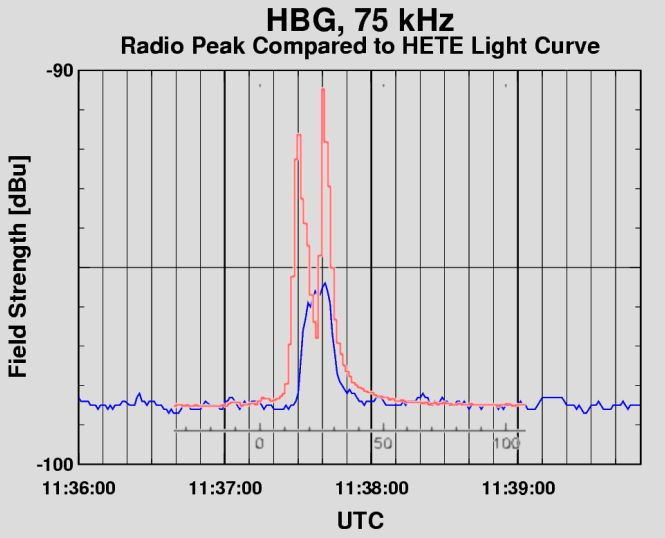
\includegraphics[width=0.49\textwidth]{figures/grb030329-prompt.jpg}
    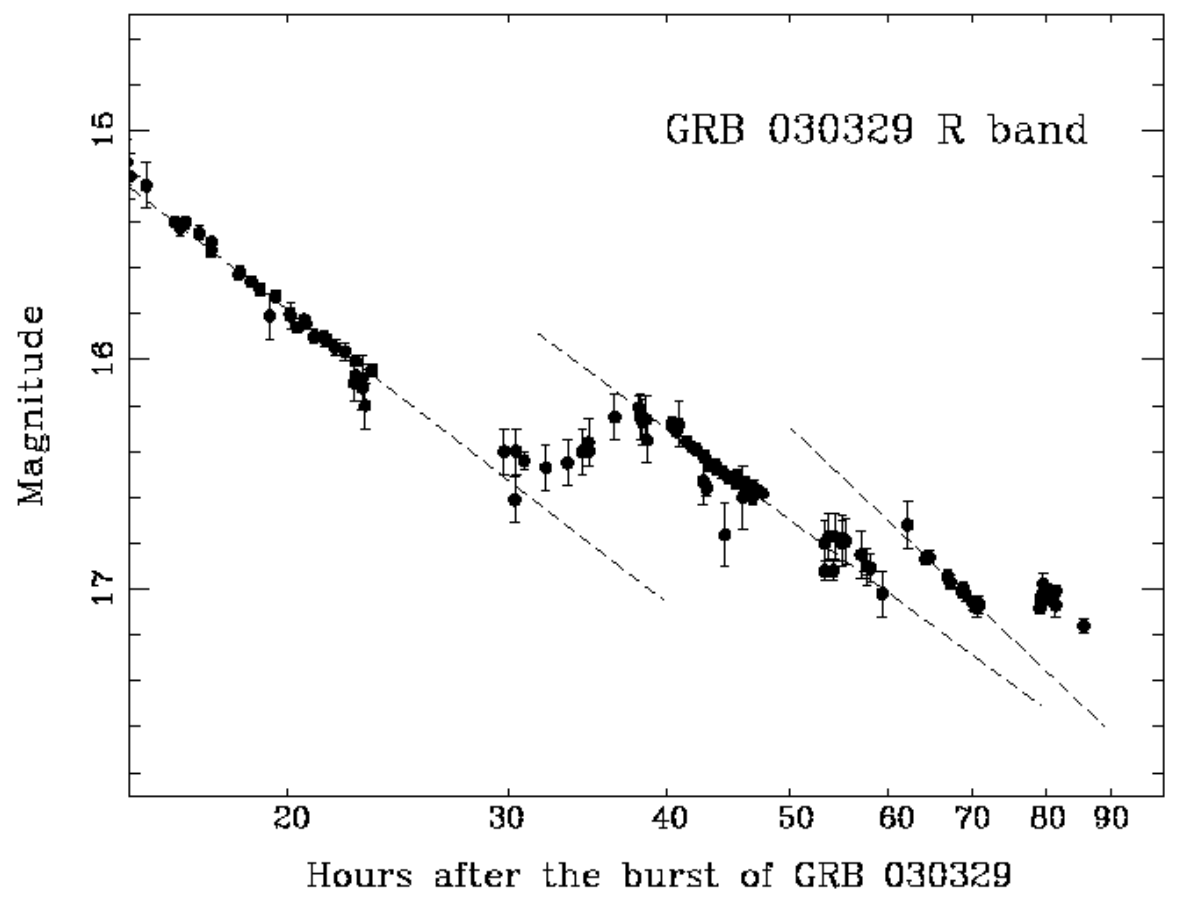
\includegraphics[width=0.49\textwidth]{figures/GRB030329-afterglow.png}
    \caption{The (a) prompt (in pink) and (b) afterglow light curves of GRB030329.}
    \label{fig: GRB030329 light curves}
\end{figure}

\newpage
\bibliographystyle{aasjournal}
\bibliography{bibliograpy-list}


\end{document}
